\chapter{System Development}

\section{Design}

System design is covered here with the intent of allowing for future modification or reproduction of the flow system. Development of neither the labVIEW Virtual Interface (VI), arduino code, nor electrical schematic are covered in detail but are presented in the attached appendixes.

\qquad


High level design inputs may be summarized as follows:


\begin{enumerate}
\item The flow system shall be controlled by a labVIEW VI.
\item The flow system shall feature four discrete pressure channels.
\item The flow system shall be capable of producing pressure output 
from 0 to 1 bar.
\item The resulting controlled pressure shall be visible to and recordable by the user.
\end{enumerate}

\qquad


In order to develop a system capable of meeting these design inputs several key components are required and those components used are specified in Table

\qquad

 
\begin{tabular}{l*{6}{c}r}
Component & Manufacturer & Part Number & Quantity \\
\hline
Regulators & Marsh Bellofram & Type 2000 & 4 \\
Transducers & AMS & 5915-1000-D & 4\\
Transducers & AMS & 5915-0350-D & 4\\
DACs & AMS & 0.014 & 54.53\\
Microcontroller & 0.043 & 0.018 & 48.14 \\
\caption[Droplet Polydispersity]{Dimensional analysis of droplets}
\label{tab:components} 
\end{tabular}


Alternative components may be acceptable, even superior, to those detailed here. Specifically, pressure transducers that allow for faster modulation may be sought.

The system electronics are self-contained within a XX rated enclosure. The system functions as a 'black box' with the 240VAC$->$9VDC power input, USB communication, main pneumatic supply line input, and 4 discrete pneumatic outputs.

\begin{figure}[H]
\centering 
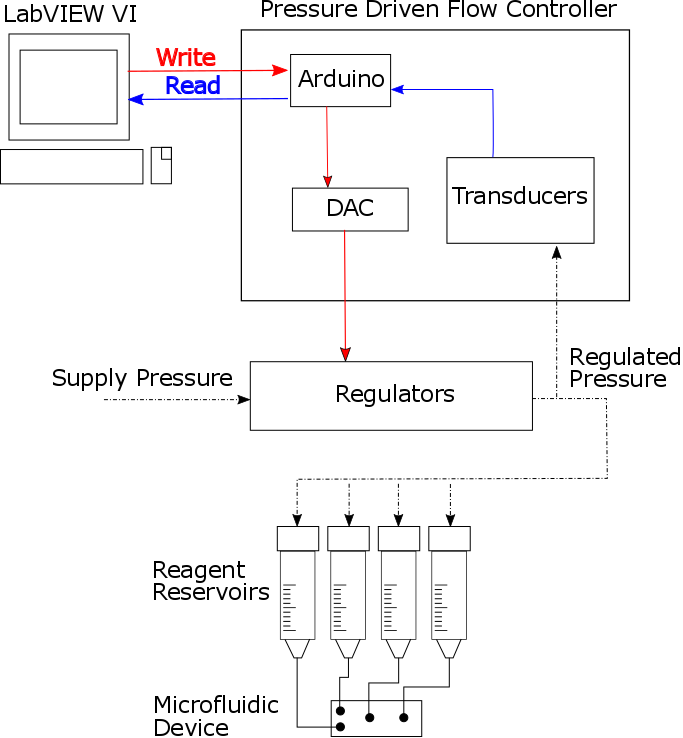
\includegraphics[width=01.0\columnwidth]{systemOverview.PNG} 
\caption[Communications flowchart for operation of the PDFC]{The control loop used to set and measure channel pressures using the PDFC} 
\label{fig:systemOverview} 
\end{figure}

The pneumatic schematic for a single channel is shown in Figure \vref{pneumaticSchematic.PNG}. Note that the air supply here is expected to be filtered to XXperc humidity and 3 micron particle filtration. 

\begin{figure}[H]
\centering 
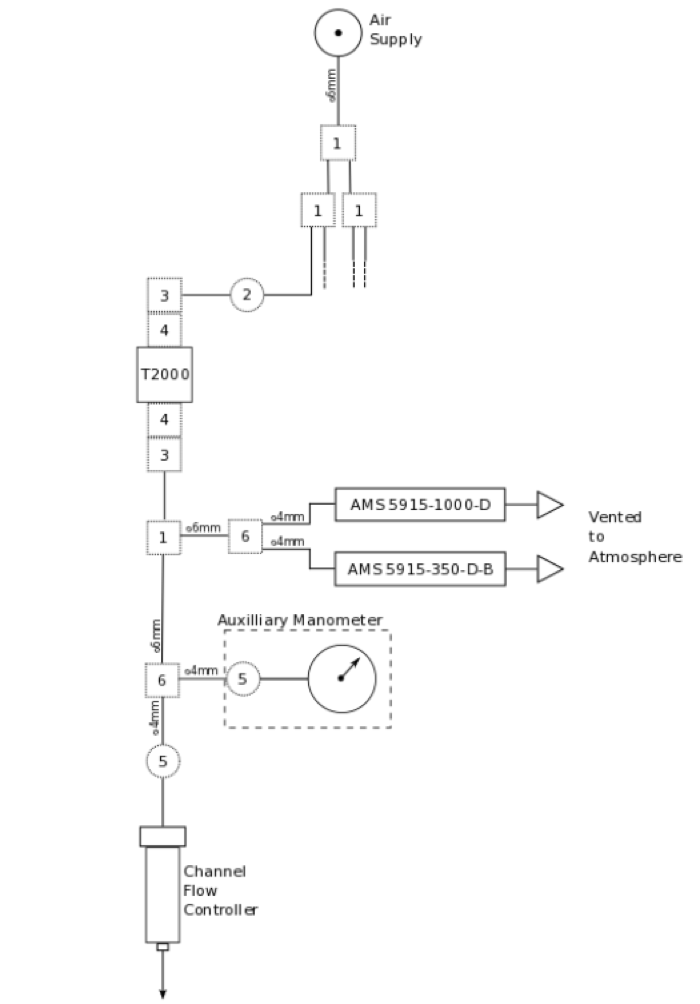
\includegraphics[width=01.0\columnwidth]{pneumaticSchematic.PNG} 
\caption[Pneumatic Schematic of PDFC channel]{The pneumatic schematic detailing a single channel of the PDFC} 
\label{fig:pneumaticSchematic} 
\end{figure}

\section{Characterization}


After completing manufacture and integration of the PDFC it must be validated prior to being used as a research tool. Particular emphasis is placed on two operating criteria of the system:
\begin{enumerate}
\item The response time of the system, from application of write signal to regulated pressure response.
\item The accuracy and channel-to-channel variance observed in the system.
\end{enumerate}

In regards to the response time of the system it may be valuable to detail the individual process steps required from signal input to response output. The user would manually enter a control signal within the labVIEW interface of 0 to 5 volts. After initiating the write command by clicking a 'write' button within the labVIEW interface, the command is written synchronously to the microcontroller via Universal Serial Bus (USB). The signal is intially sent and interpreted as a string and is processed via the embedded microcontroller code into a binary command comprised of the 4 configuration bits and 12 data bits. This binary command is then written to the Digitial Analouge Converters (DACs) via standard SPI protocol. The DACs convert the binary commands into  continuous analogue outputs capable of covering the complete pressure output of 0 to 1000 mbar.

The labVIEW VI is capable of recording the measured regulated pressure outputs, which may be used to document control pressures employed for specific experimentation. Here, that data logging capability is used to investigate the system's time response, as shown in Figure \vref{fig:timeResponse}. The gap in data is due to use of 'synchronous' USB communication. The rightmost data prior to the gap coincides with the time point at which the command signal is sent. While all channel outputs clearly converge to the desired nominal output pressure, the time response is broadly speaking slow, and variation in channel regulation is apparent as the pressure output stabilizes. Variation in the stabilization of regulated signal is due to variance from regulator to regulator. The model of regulator used here relies on a Proportional Integral Differential (PID) control circuit with manually adjustable potentiometers to adjust gain constants, non-ideal when attempting to produce coincident outputs on discrete channels.

The time from signal write to that of reaching $95\%$ of the desired output, $\tau$, increases as a function of differential pressure sought but is roughly on the magnitude of $~1 sec$. 

\begin{figure}[H]
\centering 
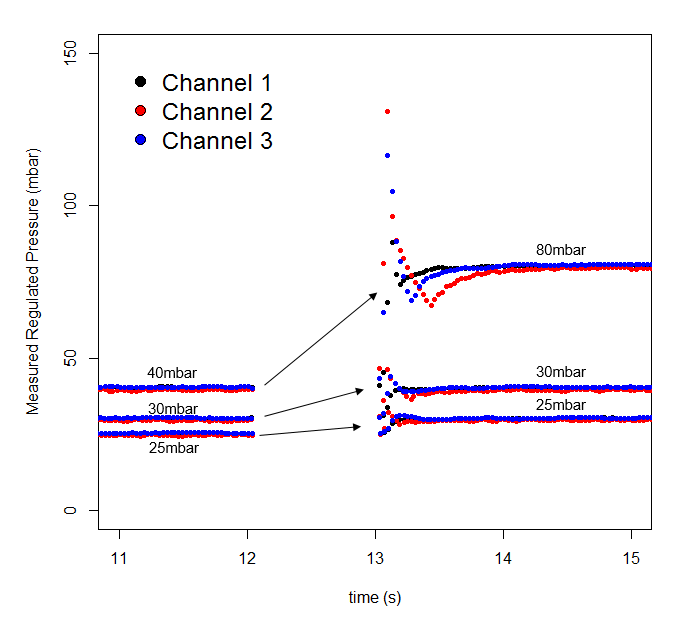
\includegraphics[width=01.0\columnwidth]{timeResponse.PNG} 
\caption[PDFC time response]{Three pressure transitions are shown, 40 to 80mbar, 30 to 40mbar, and 25 to 30mbar for 3 discrete output channels. } 
\label{fig:timeResponse} 
\end{figure}

These observations suggests that the system as currently developed is not appropriate for the millisecond or faster response times required for real-time manipulation of droplet size. This agrees with previous findings. Flow rate control of droplet formation is known for its slow response whether by syringe pump or pressure flow. Furthermore, response time of the actual device is further delayed due to fluidic capacitance caused by the compressibility of reagents, tubing and PDMS channels \cite{Churski2013,Stone2004}. If fast-response times are sought a more appropriate methodology may be to maintain a steady flowrate and drive droplet formation by active methods through direct manipulation of the fluid at the local point of formation by electrical, mechanical, magnetic, or acoustic means \cite{Chong2016}.


System accuracy and channel to channel variation can be investigated in a similar method to time response. Here, three channels are simultaneously regulated to a nominal 100mbar. After a stabilization time of approximately 3 seconds, a 15 second mean and standard deviation are acquired for each channel, as shown in area between the dashed lines in Figure \vref{fig:constV}. Each channel is capable of regulating to the nominal 100 $\pm$ 1 mbar with a standard deviation of less than 0.25 mbar.


\begin{figure}[H]
\centering 
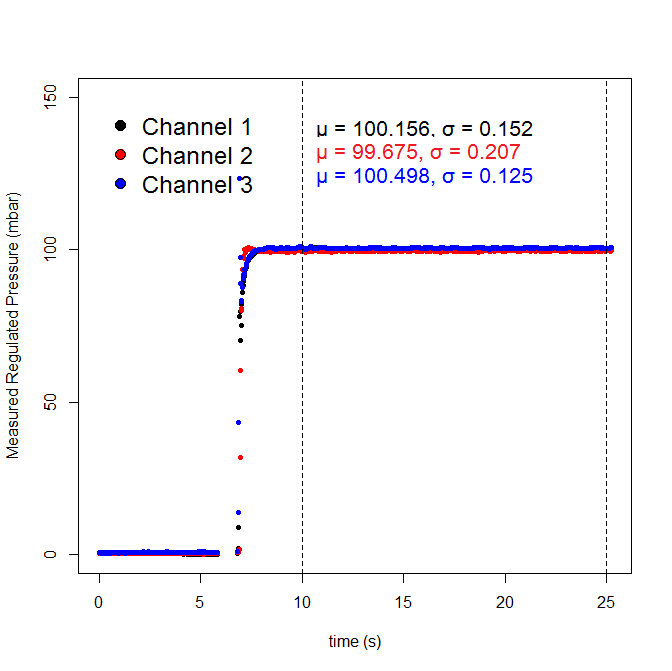
\includegraphics[width=01.0\columnwidth]{constV.PNG} 
\caption[PDFC accuracy and inter-channel variation]{Accuracy and channel-to-channel variation of the PDFC system.} 
\label{fig:constV} 
\end{figure}